\section{Method}
\label{sec:method}
\subsection{Decision Representation}
A decision example consists of a context $s$, an instruction $u$, an ordered list of candidates $\mathcal{C}=\{(k_i,d_i)\}_{i=1}^{K}$, and a target probability vector $\mathbf{y}\in\Delta^{K-1}$. Here $k_i$ is an application-facing key, $d_i$ its natural-language description, and $2\leq K\leq26$. Hard labels are one-hot vectors; soft labels retain the upstream distribution. Input validation requires finite, nonnegative targets with total mass one up to a numerical tolerance.

The interface has three question types. \noul{} is a proposition judgment with candidates ordered as false and true; its scalar result is $p(\mathrm{true})$. \choice{} returns the key with the largest probability. \score{} takes rating levels in increasing order and returns
\begin{equation}
\hat r=\sum_{i=1}^{K}(i-1)p_i.
\label{eq:score}
\end{equation}
The full distribution is retained in all cases. This expectation treats adjacent level indices as equally spaced; it does not establish equal semantic distance between arbitrary rating descriptions.

\subsection{Shared Prompt Compilation}
The compiler associates candidates with the letters A through Z, renders the context, question, candidate keys and descriptions, and applies the backbone's chat template with thinking disabled. Training, benchmarking, and serving call the same compiler, identified as \texttt{hmm-zh-v1}. Appendix~\ref{app:prompt} gives an English translation of its Chinese user-message body.

The implementation accepts at most 16,384 input tokens. Training explicitly counts and filters overlength examples; evaluation fails on overflow and serving rejects overlength requests. The full benchmark runs reported here have zero filtered or truncated decisions. This implementation limit is distinct from the backbone's native context capacity.

\begin{figure*}[t]
\centering
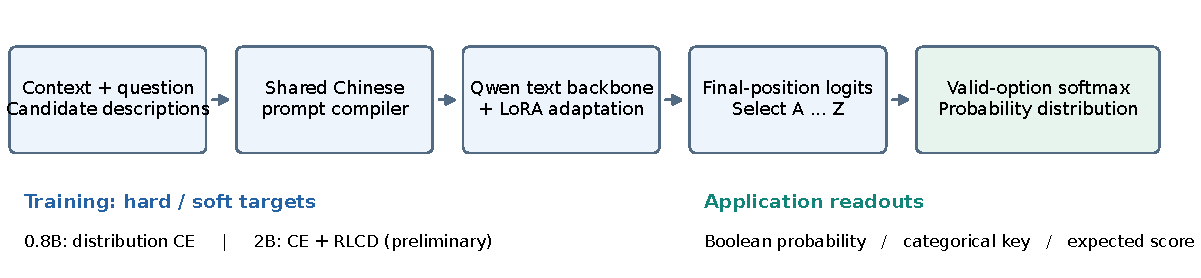
\includegraphics[width=\textwidth]{figures/pipeline.pdf}
\caption{The shared decision path. Each compiled question is evaluated once. Candidate-letter logits are normalized only over valid candidates. Training supplies hard or soft target distributions; deployment maps the same probabilities to a Boolean result, a categorical key, or an expected ordinal score. Multiple questions can be batched, but remain distinct compiled inputs.}
\label{fig:pipeline}
\end{figure*}

\subsection{Single-Pass Candidate Probabilities}
Let $x=\phi(s,u,\mathcal{C})$ be the tokenized prompt of length $L$. A causal language model produces vocabulary logits $\mathbf{v}_{L}\in\R^{|V|}$ at the final position. If $t_i$ is the token ID for candidate letter $i$, we select $z_i=v_{L,t_i}$ and compute
\begin{equation}
p_i(\mathbf{z};T)=\frac{\exp(z_i/T)}{\sum_{j=1}^{K}\exp(z_j/T)},\qquad T>0.
\label{eq:softmax}
\end{equation}
The tokenizer is checked to ensure that every candidate letter is a single token. Invalid letters are masked before normalization. The output is conditioned on the provided candidate set and excludes vocabulary mass assigned to other tokens. These are decision probabilities learned under candidate supervision, rather than unrestricted next-token probabilities or probabilities of open-ended answer correctness.

Only final-position language-model logits are requested from the backbone. The input sequence still passes through its full text network. The method removes iterative answer generation; it does not remove prompt processing or guarantee lower latency than a compact encoder.

\subsection{Distribution Supervision and LoRA}
The completed 0.8B member minimizes distribution cross-entropy:
\begin{equation}
\CE(\theta)=-\frac{1}{N}\sum_{n=1}^{N}\sum_{i=1}^{K_n}y_{ni}\log p_{\theta,i}(x_n;1).
\label{eq:ce}
\end{equation}
Because $\mathbf{y}$ may be soft, this objective retains information discarded by replacing every target with its argmax. For fixed targets it differs from $D_{\mathrm{KL}}(\mathbf{y}\Vert\mathbf{p})$ only by target entropy. It does not explicitly penalize ordinal distance between rating levels.

For a frozen backbone matrix $W_0$, LoRA learns $W=W_0+(\alpha/r)BA$. Both reported model sizes use rank $r=32$, $\alpha=64$, and dropout 0.05. Adapters target full-attention, linear-attention, and feed-forward projections. The released 0.8B weights merge the selected adapter into the backbone; Appendix~\ref{app:reproduce} lists the target modules.

During training, \choice{} candidates and their target probabilities are jointly permuted. \noul{} retains false/true order and \score{} retains level order. Permutation augmentation is intended to reduce dependence on categorical candidate position, but the experiments below do not measure permutation invariance directly.

\subsection{RLCD in the Preliminary 2B Run}
\label{sec:rlcd}
The 2B run adds an RLCD term adapted from the upstream implementation. For logits $\mathbf{z}$, it samples $M=4$ Gaussian perturbations, centers each perturbation over valid candidates, and forms
\begin{equation}
\mathbf{z}^{(m)}=\operatorname{sg}(\mathbf{z})+\tilde{\boldsymbol\epsilon}^{(m)},
\quad \mathbf{q}^{(m)}=\operatorname{softmax}(\mathbf{z}^{(m)}),
\end{equation}
where $\operatorname{sg}$ stops gradients. The reward combines a clipped log score, a spherical score, and a ranked probability score for ordinal questions:
\begin{align}
R(\mathbf{q},\mathbf{y})={}&\sum_i y_i\max(\log q_i,-9.21)\nonumber\\
&+0.75\frac{\mathbf{y}^{\top}\mathbf{q}}{\|\mathbf{q}\|_2}
-\ind_{\score}\operatorname{RPS}(\mathbf{q},\mathbf{y}),\label{eq:reward}\\
\operatorname{RPS}(\mathbf{q},\mathbf{y})={}&\frac{1}{K-1}\sum_{k=1}^{K}
\left(\sum_{i=1}^{k}(q_i-y_i)\right)^2.\label{eq:rps}
\end{align}
The final cumulative term is zero for normalized distributions. The implementation uses small numerical floors in logarithms and norms. Because the logarithmic reward is clipped, we make no blanket claim that the implemented composite reward is strictly proper over the entire probability simplex.

Let $A_m$ be the reward after subtracting the per-example perturbation-group mean. Advantages are divided by their standard deviation over the perturbation-by-microbatch tensor plus $10^{-6}$ and detached. The surrogate is
\begin{align}
\mathcal{L}_{\mathrm{RLCD}}&=-\frac1M\sum_m\operatorname{sg}(A_m)\ell_m(\mathbf{z}),\\
\ell_m(\mathbf{z})&=-\frac{\|\mathbf{z}^{(m)}-\mathbf{z}\|_2^2}{2\sigma^2},\label{eq:rlcd}
\end{align}
with an additional average over examples. The 2B objective is $\CE+\mathcal{L}_{\mathrm{RLCD}}$, with unit weights. The noise scale decreases linearly from 0.4 to 0.1 with the fraction of the planned epoch consumed. All completed 0.8B results use cross-entropy alone. Thus 0.8B--2B comparisons change both size and objective.

\subsection{Held-Out Temperature and Output Semantics}
\label{sec:temperature}
The official validation split is partitioned by a deterministic hash of parent-record identity. Four of five hash buckets are eligible for model selection; the remaining bucket is reserved for temperature fitting. Reservoir sampling selects up to 100 decisions per domain/type stratum for selection, yielding 1,200 examples. Checkpoints are chosen by distribution negative log-likelihood (NLL), not test accuracy or ECE.

For the 0.8B release, a scalar temperature is fitted on hard labels sampled from the reserved bucket by minimizing cross-entropy. This produces $T=1.108133$ from 1,993 hard-labeled calibration decisions. No test labels are used for fitting. We report $T=1$ for main checkpoint comparisons and use the fixed fitted temperature only in the deployment study.

The API also returns a normalized sharpness statistic
\begin{equation}
c=\frac{K\max_i p_i-1}{K-1}.\label{eq:confidence}
\end{equation}
It is zero for a uniform distribution and one for a point mass. It is not an empirical correctness probability. Benchmark ECE uses $\max_i p_i$, not $c$.
